\documentclass[1p]{elsarticle_modified}
%\bibliographystyle{elsarticle-num}

%\usepackage[colorlinks]{hyperref}
%\usepackage{abbrmath_seonhwa} %\Abb, \Ascr, \Acal ,\Abf, \Afrak
\usepackage{amsfonts}
\usepackage{amssymb}
\usepackage{amsmath}
\usepackage{amsthm}
\usepackage{scalefnt}
\usepackage{amsbsy}
\usepackage{kotex}
\usepackage{caption}
\usepackage{subfig}
\usepackage{color}
\usepackage{graphicx}
\usepackage{xcolor} %% white, black, red, green, blue, cyan, magenta, yellow
\usepackage{float}
\usepackage{setspace}
\usepackage{hyperref}

\usepackage{tikz}
\usetikzlibrary{arrows}

\usepackage{multirow}
\usepackage{array} % fixed length table
\usepackage{hhline}

%%%%%%%%%%%%%%%%%%%%%
\makeatletter
\renewcommand*\env@matrix[1][\arraystretch]{%
	\edef\arraystretch{#1}%
	\hskip -\arraycolsep
	\let\@ifnextchar\new@ifnextchar
	\array{*\c@MaxMatrixCols c}}
\makeatother %https://tex.stackexchange.com/questions/14071/how-can-i-increase-the-line-spacing-in-a-matrix
%%%%%%%%%%%%%%%

\usepackage[normalem]{ulem}

\newcommand{\msout}[1]{\ifmmode\text{\sout{\ensuremath{#1}}}\else\sout{#1}\fi}
%SOURCE: \msout is \stkout macro in https://tex.stackexchange.com/questions/20609/strikeout-in-math-mode

\newcommand{\cancel}[1]{
	\ifmmode
	{\color{red}\msout{#1}}
	\else
	{\color{red}\sout{#1}}
	\fi
}

\newcommand{\add}[1]{
	{\color{blue}\uwave{#1}}
}

\newcommand{\replace}[2]{
	\ifmmode
	{\color{red}\msout{#1}}{\color{blue}\uwave{#2}}
	\else
	{\color{red}\sout{#1}}{\color{blue}\uwave{#2}}
	\fi
}

\newcommand{\Sol}{\mathcal{S}} %segment
\newcommand{\D}{D} %diagram
\newcommand{\A}{\mathcal{A}} %arc


%%%%%%%%%%%%%%%%%%%%%%%%%%%%%5 test

\def\sl{\operatorname{\textup{SL}}(2,\Cbb)}
\def\psl{\operatorname{\textup{PSL}}(2,\Cbb)}
\def\quan{\mkern 1mu \triangleright \mkern 1mu}

\theoremstyle{definition}
\newtheorem{thm}{Theorem}[section]
\newtheorem{prop}[thm]{Proposition}
\newtheorem{lem}[thm]{Lemma}
\newtheorem{ques}[thm]{Question}
\newtheorem{cor}[thm]{Corollary}
\newtheorem{defn}[thm]{Definition}
\newtheorem{exam}[thm]{Example}
\newtheorem{rmk}[thm]{Remark}
\newtheorem{alg}[thm]{Algorithm}

\newcommand{\I}{\sqrt{-1}}
\begin{document}

%\begin{frontmatter}
%
%\title{Boundary parabolic representations of knots up to 8 crossings}
%
%%% Group authors per affiliation:
%\author{Yunhi Cho} 
%\address{Department of Mathematics, University of Seoul, Seoul, Korea}
%\ead{yhcho@uos.ac.kr}
%
%
%\author{Seonhwa Kim} %\fnref{s_kim}}
%\address{Center for Geometry and Physics, Institute for Basic Science, Pohang, 37673, Korea}
%\ead{ryeona17@ibs.re.kr}
%
%\author{Hyuk Kim}
%\address{Department of Mathematical Sciences, Seoul National University, Seoul 08826, Korea}
%\ead{hyukkim@snu.ac.kr}
%
%\author{Seokbeom Yoon}
%\address{Department of Mathematical Sciences, Seoul National University, Seoul, 08826,  Korea}
%\ead{sbyoon15@snu.ac.kr}
%
%\begin{abstract}
%We find all boundary parabolic representation of knots up to 8 crossings.
%
%\end{abstract}
%\begin{keyword}
%    \MSC[2010] 57M25 
%\end{keyword}
%
%\end{frontmatter}

%\linenumbers
%\tableofcontents
%
\newcommand\colored[1]{\textcolor{white}{\rule[-0.35ex]{0.8em}{1.4ex}}\kern-0.8em\color{red} #1}%
%\newcommand\colored[1]{\textcolor{white}{ #1}\kern-2.17ex	\textcolor{white}{ #1}\kern-1.81ex	\textcolor{white}{ #1}\kern-2.15ex\color{red}#1	}

{\Large $\underline{10_{80}~(K10a_{8})}$}

\setlength{\tabcolsep}{10pt}
\renewcommand{\arraystretch}{1.6}
\vspace{1cm}\begin{tabular}{m{100pt}>{\centering\arraybackslash}m{274pt}}
\multirow{5}{120pt}{
	\centering
	\includegraphics[width=112pt]{../../../GIT/diagram.site/Diagrams/png/164_10_80.png}\\
\ \ \ A knot diagram\footnotemark}&
\allowdisplaybreaks
\textbf{Linearized knot diagam} \\
\cline{2-2}
 &
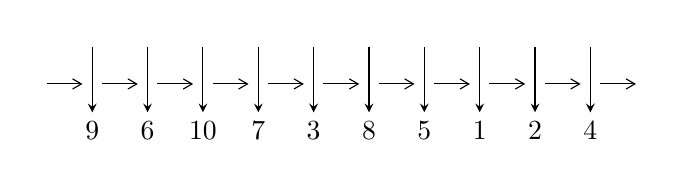
\begin{tikzpicture}[x=20pt, y=17pt]
	% nodes
	\node (C0) at (0, 0) {};
	\node (C1) at (1, 0) {};
	\node (C1U) at (1, +1) {};
	\node (C1D) at (1, -1) {9};

	\node (C2) at (2, 0) {};
	\node (C2U) at (2, +1) {};
	\node (C2D) at (2, -1) {6};

	\node (C3) at (3, 0) {};
	\node (C3U) at (3, +1) {};
	\node (C3D) at (3, -1) {10};

	\node (C4) at (4, 0) {};
	\node (C4U) at (4, +1) {};
	\node (C4D) at (4, -1) {7};

	\node (C5) at (5, 0) {};
	\node (C5U) at (5, +1) {};
	\node (C5D) at (5, -1) {3};

	\node (C6) at (6, 0) {};
	\node (C6U) at (6, +1) {};
	\node (C6D) at (6, -1) {8};

	\node (C7) at (7, 0) {};
	\node (C7U) at (7, +1) {};
	\node (C7D) at (7, -1) {5};

	\node (C8) at (8, 0) {};
	\node (C8U) at (8, +1) {};
	\node (C8D) at (8, -1) {1};

	\node (C9) at (9, 0) {};
	\node (C9U) at (9, +1) {};
	\node (C9D) at (9, -1) {2};

	\node (C10) at (10, 0) {};
	\node (C10U) at (10, +1) {};
	\node (C10D) at (10, -1) {4};
	\node (C11) at (11, 0) {};

	% arrows
	\draw[->,>={angle 60}]
	(C0) edge (C1) (C1) edge (C2) (C2) edge (C3) (C3) edge (C4) (C4) edge (C5) (C5) edge (C6) (C6) edge (C7) (C7) edge (C8) (C8) edge (C9) (C9) edge (C10) (C10) edge (C11) ;	\draw[->,>=stealth]
	(C1U) edge (C1D) (C2U) edge (C2D) (C3U) edge (C3D) (C4U) edge (C4D) (C5U) edge (C5D) (C6U) edge (C6D) (C7U) edge (C7D) (C8U) edge (C8D) (C9U) edge (C9D) (C10U) edge (C10D) ;
	\end{tikzpicture} \\
\hhline{~~} \\& 
\textbf{Solving Sequence} \\ \cline{2-2} 
 &
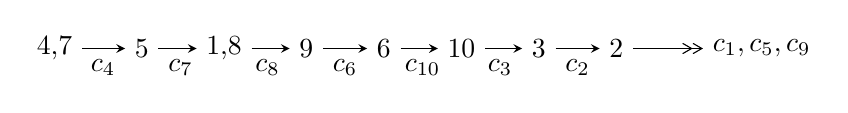
\begin{tikzpicture}[x=28pt, y=7pt]
	% node
	\node (A0) at (-1/8, 0) {4,7};
	\node (A1) at (1, 0) {5};
	\node (A2) at (33/16, 0) {1,8};
	\node (A3) at (25/8, 0) {9};
	\node (A4) at (33/8, 0) {6};
	\node (A5) at (41/8, 0) {10};
	\node (A6) at (49/8, 0) {3};
	\node (A7) at (57/8, 0) {2};
	\node (C1) at (1/2, -1) {$c_{4}$};
	\node (C2) at (3/2, -1) {$c_{7}$};
	\node (C3) at (21/8, -1) {$c_{8}$};
	\node (C4) at (29/8, -1) {$c_{6}$};
	\node (C5) at (37/8, -1) {$c_{10}$};
	\node (C6) at (45/8, -1) {$c_{3}$};
	\node (C7) at (53/8, -1) {$c_{2}$};
	\node (A8) at (9, 0) {$c_{1},c_{5},c_{9}$};

	% edge
	\draw[->,>=stealth]	
	(A0) edge (A1) (A1) edge (A2) (A2) edge (A3) (A3) edge (A4) (A4) edge (A5) (A5) edge (A6) (A6) edge (A7) ;
	\draw[->>,>={angle 60}]	
	(A7) edge (A8);
\end{tikzpicture} \\ 

\end{tabular} \\

\footnotetext{
The image of knot diagram is generated by the software ``\textbf{Draw programme}" developed by Andrew Bartholomew(\url{http://www.layer8.co.uk/maths/draw/index.htm\#Running-draw}), where we modified some parts for our purpose(\url{https://github.com/CATsTAILs/LinksPainter}).
}\phantom \\ \newline 
\centering \textbf{Ideals for irreducible components\footnotemark of $X_{\text{par}}$} 
 
\begin{align*}
I^u_{1}&=\langle 
1794841722415 u^{39}+5490595544415 u^{38}+\cdots+1305995790962 b+2649665691745,\\
\phantom{I^u_{1}}&\phantom{= \langle  }-1190941729941 u^{39}-4615935344485 u^{38}+\cdots+1305995790962 a-3386435539405,\\
\phantom{I^u_{1}}&\phantom{= \langle  }u^{40}+4 u^{39}+\cdots-2 u+1\rangle \\
I^u_{2}&=\langle 
b,\;u^2+a+2 u+1,\;u^3+u^2-1\rangle \\
I^u_{3}&=\langle 
b- a-1,\;a^2+a-1,\;u-1\rangle \\
\\
\end{align*}
\raggedright * 3 irreducible components of $\dim_{\mathbb{C}}=0$, with total 45 representations.\\
\footnotetext{All coefficients of polynomials are rational numbers. But the coefficients are sometimes approximated in decimal forms when there is not enough margin.}
\newpage
\renewcommand{\arraystretch}{1}
\centering \section*{I. $I^u_{1}= \langle 1.79\times10^{12} u^{39}+5.49\times10^{12} u^{38}+\cdots+1.31\times10^{12} b+2.65\times10^{12},\;-1.19\times10^{12} u^{39}-4.62\times10^{12} u^{38}+\cdots+1.31\times10^{12} a-3.39\times10^{12},\;u^{40}+4 u^{39}+\cdots-2 u+1 \rangle$}
\flushleft \textbf{(i) Arc colorings}\\
\begin{tabular}{m{7pt} m{180pt} m{7pt} m{180pt} }
\flushright $a_{4}=$&$\begin{pmatrix}1\\0\end{pmatrix}$ \\
\flushright $a_{7}=$&$\begin{pmatrix}0\\u\end{pmatrix}$ \\
\flushright $a_{5}=$&$\begin{pmatrix}1\\u^2\end{pmatrix}$ \\
\flushright $a_{1}=$&$\begin{pmatrix}0.911903 u^{39}+3.53442 u^{38}+\cdots+4.75622 u+2.59299\\-1.37431 u^{39}-4.20414 u^{38}+\cdots+3.79441 u-2.02885\end{pmatrix}$ \\
\flushright $a_{8}=$&$\begin{pmatrix}- u\\- u^3+u\end{pmatrix}$ \\
\flushright $a_{9}=$&$\begin{pmatrix}-2.36296 u^{39}-8.30641 u^{38}+\cdots+1.11511 u-2.81278\\0.625691 u^{39}+1.79586 u^{38}+\cdots-1.20559 u+0.971153\end{pmatrix}$ \\
\flushright $a_{6}=$&$\begin{pmatrix}u^3\\u^5- u^3+u\end{pmatrix}$ \\
\flushright $a_{10}=$&$\begin{pmatrix}-0.462406 u^{39}-0.669727 u^{38}+\cdots+8.55064 u+0.564144\\-1.37431 u^{39}-4.20414 u^{38}+\cdots+3.79441 u-2.02885\end{pmatrix}$ \\
\flushright $a_{3}=$&$\begin{pmatrix}-0.481242 u^{39}-1.19932 u^{38}+\cdots+3.81151 u+1.61679\\-1.34743 u^{39}-3.78400 u^{38}+\cdots+3.42400 u-1.70725\end{pmatrix}$ \\
\flushright $a_{2}=$&$\begin{pmatrix}-2.58732 u^{39}-8.51193 u^{38}+\cdots+10.6671 u-0.875683\\-0.625691 u^{39}-1.79586 u^{38}+\cdots+1.20559 u-0.971153\end{pmatrix}$\\&\end{tabular}
\flushleft \textbf{(ii) Obstruction class $= -1$}\\~\\
\flushleft \textbf{(iii) Cusp Shapes $= -\frac{1683630050026}{652997895481} u^{39}-\frac{6742803896956}{652997895481} u^{38}+\cdots-\frac{5009068136946}{652997895481} u-\frac{5965220685850}{652997895481}$}\\~\\
\newpage\renewcommand{\arraystretch}{1}
\flushleft \textbf{(iv) u-Polynomials at the component}\newline \\
\begin{tabular}{m{50pt}|m{274pt}}
Crossings & \hspace{64pt}u-Polynomials at each crossing \\
\hline $$\begin{aligned}c_{1},c_{8},c_{9}\end{aligned}$$&$\begin{aligned}
&u^{40}-5 u^{39}+\cdots+6 u+1
\end{aligned}$\\
\hline $$\begin{aligned}c_{2},c_{5}\end{aligned}$$&$\begin{aligned}
&u^{40}-2 u^{39}+\cdots+4 u-4
\end{aligned}$\\
\hline $$\begin{aligned}c_{3},c_{10}\end{aligned}$$&$\begin{aligned}
&u^{40}+2 u^{39}+\cdots-28 u-8
\end{aligned}$\\
\hline $$\begin{aligned}c_{4},c_{7}\end{aligned}$$&$\begin{aligned}
&u^{40}-4 u^{39}+\cdots+2 u+1
\end{aligned}$\\
\hline $$\begin{aligned}c_{6}\end{aligned}$$&$\begin{aligned}
&u^{40}+20 u^{39}+\cdots+38 u+1
\end{aligned}$\\
\hline
\end{tabular}\\~\\
\newpage\renewcommand{\arraystretch}{1}
\flushleft \textbf{(v) Riley Polynomials at the component}\newline \\
\begin{tabular}{m{50pt}|m{274pt}}
Crossings & \hspace{64pt}Riley Polynomials at each crossing \\
\hline $$\begin{aligned}c_{1},c_{8},c_{9}\end{aligned}$$&$\begin{aligned}
&y^{40}-39 y^{39}+\cdots+24 y+1
\end{aligned}$\\
\hline $$\begin{aligned}c_{2},c_{5}\end{aligned}$$&$\begin{aligned}
&y^{40}+18 y^{39}+\cdots-104 y+16
\end{aligned}$\\
\hline $$\begin{aligned}c_{3},c_{10}\end{aligned}$$&$\begin{aligned}
&y^{40}-24 y^{39}+\cdots-1360 y+64
\end{aligned}$\\
\hline $$\begin{aligned}c_{4},c_{7}\end{aligned}$$&$\begin{aligned}
&y^{40}-20 y^{39}+\cdots-38 y+1
\end{aligned}$\\
\hline $$\begin{aligned}c_{6}\end{aligned}$$&$\begin{aligned}
&y^{40}+4 y^{39}+\cdots-918 y+1
\end{aligned}$\\
\hline
\end{tabular}\\~\\
\newpage\flushleft \textbf{(vi) Complex Volumes and Cusp Shapes}
$$\begin{array}{c|c|c}  
\text{Solutions to }I^u_{1}& \I (\text{vol} + \sqrt{-1}CS) & \text{Cusp shape}\\
 \hline 
\begin{aligned}
u &= -0.272416 + 0.968858 I \\
a &= \phantom{-}0.945891 + 0.854682 I \\
b &= -1.224160 - 0.640097 I\end{aligned}
 & -3.73330 - 7.68923 I & -11.60024 + 4.76581 I \\ \hline\begin{aligned}
u &= -0.272416 - 0.968858 I \\
a &= \phantom{-}0.945891 - 0.854682 I \\
b &= -1.224160 + 0.640097 I\end{aligned}
 & -3.73330 + 7.68923 I & -11.60024 - 4.76581 I \\ \hline\begin{aligned}
u &= -0.645648 + 0.698758 I \\
a &= \phantom{-}0.141845 + 1.079620 I \\
b &= \phantom{-}0.488954 - 0.746861 I\end{aligned}
 & \phantom{-}3.38024 + 1.21441 I & -4.33120 - 2.38202 I \\ \hline\begin{aligned}
u &= -0.645648 - 0.698758 I \\
a &= \phantom{-}0.141845 - 1.079620 I \\
b &= \phantom{-}0.488954 + 0.746861 I\end{aligned}
 & \phantom{-}3.38024 - 1.21441 I & -4.33120 + 2.38202 I \\ \hline\begin{aligned}
u &= -1.038880 + 0.250251 I \\
a &= \phantom{-}0.485795 + 0.350283 I \\
b &= \phantom{-}1.66075 + 0.19671 I\end{aligned}
 & -10.88700 + 0.63545 I & -16.1019 - 7.3224 I \\ \hline\begin{aligned}
u &= -1.038880 - 0.250251 I \\
a &= \phantom{-}0.485795 - 0.350283 I \\
b &= \phantom{-}1.66075 - 0.19671 I\end{aligned}
 & -10.88700 - 0.63545 I & -16.1019 + 7.3224 I \\ \hline\begin{aligned}
u &= \phantom{-}0.917670\phantom{ +0.000000I} \\
a &= \phantom{-}4.22167\phantom{ +0.000000I} \\
b &= \phantom{-}0.349359\phantom{ +0.000000I}\end{aligned}
 & -2.98695\phantom{ +0.000000I} & -59.3920\phantom{ +0.000000I} \\ \hline\begin{aligned}
u &= \phantom{-}1.033250 + 0.435364 I \\
a &= -0.60097 + 1.79230 I \\
b &= -0.986819 - 0.340805 I\end{aligned}
 & -2.52882 - 3.14028 I & -13.2871 + 4.9220 I \\ \hline\begin{aligned}
u &= \phantom{-}1.033250 - 0.435364 I \\
a &= -0.60097 - 1.79230 I \\
b &= -0.986819 + 0.340805 I\end{aligned}
 & -2.52882 + 3.14028 I & -13.2871 - 4.9220 I \\ \hline\begin{aligned}
u &= \phantom{-}0.424088 + 0.764374 I \\
a &= -1.58059 + 0.54433 I \\
b &= \phantom{-}1.213240 - 0.287237 I\end{aligned}
 & -6.42531 + 1.37910 I & -14.4871 - 0.1126 I\\
 \hline 
 \end{array}$$\newpage$$\begin{array}{c|c|c}  
\text{Solutions to }I^u_{1}& \I (\text{vol} + \sqrt{-1}CS) & \text{Cusp shape}\\
 \hline 
\begin{aligned}
u &= \phantom{-}0.424088 - 0.764374 I \\
a &= -1.58059 - 0.54433 I \\
b &= \phantom{-}1.213240 + 0.287237 I\end{aligned}
 & -6.42531 - 1.37910 I & -14.4871 + 0.1126 I \\ \hline\begin{aligned}
u &= -0.334699 + 0.793502 I \\
a &= -0.423088 - 0.639117 I \\
b &= \phantom{-}1.031810 + 0.544946 I\end{aligned}
 & \phantom{-}1.73108 - 3.69196 I & -7.37427 + 4.06105 I \\ \hline\begin{aligned}
u &= -0.334699 - 0.793502 I \\
a &= -0.423088 + 0.639117 I \\
b &= \phantom{-}1.031810 - 0.544946 I\end{aligned}
 & \phantom{-}1.73108 + 3.69196 I & -7.37427 - 4.06105 I \\ \hline\begin{aligned}
u &= \phantom{-}1.096340 + 0.338707 I \\
a &= -1.05201 + 1.21469 I \\
b &= \phantom{-}0.110133 - 0.969437 I\end{aligned}
 & -4.81110 - 1.15004 I & -14.8249 + 0.1630 I \\ \hline\begin{aligned}
u &= \phantom{-}1.096340 - 0.338707 I \\
a &= -1.05201 - 1.21469 I \\
b &= \phantom{-}0.110133 + 0.969437 I\end{aligned}
 & -4.81110 + 1.15004 I & -14.8249 - 0.1630 I \\ \hline\begin{aligned}
u &= -0.955160 + 0.637303 I \\
a &= -0.565833 - 0.448992 I \\
b &= \phantom{-}0.220904 + 0.771822 I\end{aligned}
 & \phantom{-}2.47440 + 3.90124 I & -5.43445 - 4.68146 I \\ \hline\begin{aligned}
u &= -0.955160 - 0.637303 I \\
a &= -0.565833 + 0.448992 I \\
b &= \phantom{-}0.220904 - 0.771822 I\end{aligned}
 & \phantom{-}2.47440 - 3.90124 I & -5.43445 + 4.68146 I \\ \hline\begin{aligned}
u &= -1.048110 + 0.492760 I \\
a &= -0.904373 - 0.926403 I \\
b &= -1.239580 + 0.203806 I\end{aligned}
 & -2.11016 + 3.32020 I & -13.06049 - 3.76837 I \\ \hline\begin{aligned}
u &= -1.048110 - 0.492760 I \\
a &= -0.904373 + 0.926403 I \\
b &= -1.239580 - 0.203806 I\end{aligned}
 & -2.11016 - 3.32020 I & -13.06049 + 3.76837 I \\ \hline\begin{aligned}
u &= \phantom{-}1.160490 + 0.215401 I \\
a &= \phantom{-}1.009060 - 0.552611 I \\
b &= \phantom{-}0.895187 - 0.176420 I\end{aligned}
 & -3.04518 + 0.83928 I & -13.6876 - 5.4055 I\\
 \hline 
 \end{array}$$\newpage$$\begin{array}{c|c|c}  
\text{Solutions to }I^u_{1}& \I (\text{vol} + \sqrt{-1}CS) & \text{Cusp shape}\\
 \hline 
\begin{aligned}
u &= \phantom{-}1.160490 - 0.215401 I \\
a &= \phantom{-}1.009060 + 0.552611 I \\
b &= \phantom{-}0.895187 + 0.176420 I\end{aligned}
 & -3.04518 - 0.83928 I & -13.6876 + 5.4055 I \\ \hline\begin{aligned}
u &= -1.109770 + 0.525691 I \\
a &= \phantom{-}0.749622 + 0.680872 I \\
b &= -0.374879 - 1.281230 I\end{aligned}
 & -3.50534 + 6.28261 I & -13.0953 - 5.4809 I \\ \hline\begin{aligned}
u &= -1.109770 - 0.525691 I \\
a &= \phantom{-}0.749622 - 0.680872 I \\
b &= -0.374879 + 1.281230 I\end{aligned}
 & -3.50534 - 6.28261 I & -13.0953 + 5.4809 I \\ \hline\begin{aligned}
u &= -0.873586 + 0.885492 I \\
a &= \phantom{-}0.722061 - 0.543762 I \\
b &= -0.840743 + 0.122050 I\end{aligned}
 & \phantom{-}0.49614 + 3.22180 I & -15.2960 - 4.0561 I \\ \hline\begin{aligned}
u &= -0.873586 - 0.885492 I \\
a &= \phantom{-}0.722061 + 0.543762 I \\
b &= -0.840743 - 0.122050 I\end{aligned}
 & \phantom{-}0.49614 - 3.22180 I & -15.2960 + 4.0561 I \\ \hline\begin{aligned}
u &= \phantom{-}1.109100 + 0.586635 I \\
a &= -0.04572 - 1.84175 I \\
b &= \phantom{-}1.281130 + 0.518288 I\end{aligned}
 & -8.48566 - 6.50843 I & -15.7623 + 4.5910 I \\ \hline\begin{aligned}
u &= \phantom{-}1.109100 - 0.586635 I \\
a &= -0.04572 + 1.84175 I \\
b &= \phantom{-}1.281130 - 0.518288 I\end{aligned}
 & -8.48566 + 6.50843 I & -15.7623 - 4.5910 I \\ \hline\begin{aligned}
u &= -1.135680 + 0.577352 I \\
a &= \phantom{-}0.73159 + 1.41035 I \\
b &= \phantom{-}1.232290 - 0.518147 I\end{aligned}
 & -0.64027 + 8.82354 I & -11.18744 - 7.65851 I \\ \hline\begin{aligned}
u &= -1.135680 - 0.577352 I \\
a &= \phantom{-}0.73159 - 1.41035 I \\
b &= \phantom{-}1.232290 + 0.518147 I\end{aligned}
 & -0.64027 - 8.82354 I & -11.18744 + 7.65851 I \\ \hline\begin{aligned}
u &= \phantom{-}0.684183 + 0.185929 I \\
a &= \phantom{-}1.011580 - 0.590171 I \\
b &= -0.399719 + 0.274052 I\end{aligned}
 & -0.945608 - 0.085520 I & -9.49008 - 0.83288 I\\
 \hline 
 \end{array}$$\newpage$$\begin{array}{c|c|c}  
\text{Solutions to }I^u_{1}& \I (\text{vol} + \sqrt{-1}CS) & \text{Cusp shape}\\
 \hline 
\begin{aligned}
u &= \phantom{-}0.684183 - 0.185929 I \\
a &= \phantom{-}1.011580 + 0.590171 I \\
b &= -0.399719 - 0.274052 I\end{aligned}
 & -0.945608 + 0.085520 I & -9.49008 + 0.83288 I \\ \hline\begin{aligned}
u &= -0.289056 + 0.640853 I \\
a &= -0.58487 - 1.93617 I \\
b &= -0.435741 + 0.971160 I\end{aligned}
 & -1.17381 - 1.71654 I & -9.22754 + 1.14237 I \\ \hline\begin{aligned}
u &= -0.289056 - 0.640853 I \\
a &= -0.58487 + 1.93617 I \\
b &= -0.435741 - 0.971160 I\end{aligned}
 & -1.17381 + 1.71654 I & -9.22754 - 1.14237 I \\ \hline\begin{aligned}
u &= -0.491493 + 0.483729 I \\
a &= -0.533644 + 0.146067 I \\
b &= -0.888256 - 0.454789 I\end{aligned}
 & -0.414732 + 0.767581 I & -9.73697 - 1.10255 I \\ \hline\begin{aligned}
u &= -0.491493 - 0.483729 I \\
a &= -0.533644 - 0.146067 I \\
b &= -0.888256 + 0.454789 I\end{aligned}
 & -0.414732 - 0.767581 I & -9.73697 + 1.10255 I \\ \hline\begin{aligned}
u &= -1.217970 + 0.609804 I \\
a &= -0.43882 - 1.60438 I \\
b &= -1.33819 + 0.73038 I\end{aligned}
 & -6.6238 + 13.3940 I & -14.1442 - 7.8976 I \\ \hline\begin{aligned}
u &= -1.217970 - 0.609804 I \\
a &= -0.43882 + 1.60438 I \\
b &= -1.33819 - 0.73038 I\end{aligned}
 & -6.6238 - 13.3940 I & -14.1442 + 7.8976 I \\ \hline\begin{aligned}
u &= \phantom{-}1.355550 + 0.252070 I \\
a &= -0.147210 + 0.232788 I \\
b &= -1.289140 + 0.415642 I\end{aligned}
 & -9.24274 + 3.54815 I & -15.7354 - 3.2017 I \\ \hline\begin{aligned}
u &= \phantom{-}1.355550 - 0.252070 I \\
a &= -0.147210 - 0.232788 I \\
b &= -1.289140 - 0.415642 I\end{aligned}
 & -9.24274 - 3.54815 I & -15.7354 + 3.2017 I \\ \hline\begin{aligned}
u &= \phantom{-}0.181281\phantom{ +0.000000I} \\
a &= \phantom{-}2.93770\phantom{ +0.000000I} \\
b &= -0.583695\phantom{ +0.000000I}\end{aligned}
 & -0.821503\phantom{ +0.000000I} & -11.8790\phantom{ +0.000000I}\\
 \hline 
 \end{array}$$\newpage\newpage\renewcommand{\arraystretch}{1}
\centering \section*{II. $I^u_{2}= \langle b,\;u^2+a+2 u+1,\;u^3+u^2-1 \rangle$}
\flushleft \textbf{(i) Arc colorings}\\
\begin{tabular}{m{7pt} m{180pt} m{7pt} m{180pt} }
\flushright $a_{4}=$&$\begin{pmatrix}1\\0\end{pmatrix}$ \\
\flushright $a_{7}=$&$\begin{pmatrix}0\\u\end{pmatrix}$ \\
\flushright $a_{5}=$&$\begin{pmatrix}1\\u^2\end{pmatrix}$ \\
\flushright $a_{1}=$&$\begin{pmatrix}- u^2-2 u-1\\0\end{pmatrix}$ \\
\flushright $a_{8}=$&$\begin{pmatrix}- u\\u^2+u-1\end{pmatrix}$ \\
\flushright $a_{9}=$&$\begin{pmatrix}- u^2-3 u-1\\u^2+u-1\end{pmatrix}$ \\
\flushright $a_{6}=$&$\begin{pmatrix}- u^2+1\\u^2\end{pmatrix}$ \\
\flushright $a_{10}=$&$\begin{pmatrix}- u^2-2 u-1\\0\end{pmatrix}$ \\
\flushright $a_{3}=$&$\begin{pmatrix}1\\0\end{pmatrix}$ \\
\flushright $a_{2}=$&$\begin{pmatrix}u\\- u^2- u+1\end{pmatrix}$\\&\end{tabular}
\flushleft \textbf{(ii) Obstruction class $= 1$}\\~\\
\flushleft \textbf{(iii) Cusp Shapes $= u^2-8$}\\~\\
\newpage\renewcommand{\arraystretch}{1}
\flushleft \textbf{(iv) u-Polynomials at the component}\newline \\
\begin{tabular}{m{50pt}|m{274pt}}
Crossings & \hspace{64pt}u-Polynomials at each crossing \\
\hline $$\begin{aligned}c_{1}\end{aligned}$$&$\begin{aligned}
&(u+1)^3
\end{aligned}$\\
\hline $$\begin{aligned}c_{2},c_{6}\end{aligned}$$&$\begin{aligned}
&u^3- u^2+2 u-1
\end{aligned}$\\
\hline $$\begin{aligned}c_{3},c_{10}\end{aligned}$$&$\begin{aligned}
&u^3
\end{aligned}$\\
\hline $$\begin{aligned}c_{4}\end{aligned}$$&$\begin{aligned}
&u^3+u^2-1
\end{aligned}$\\
\hline $$\begin{aligned}c_{5}\end{aligned}$$&$\begin{aligned}
&u^3+u^2+2 u+1
\end{aligned}$\\
\hline $$\begin{aligned}c_{7}\end{aligned}$$&$\begin{aligned}
&u^3- u^2+1
\end{aligned}$\\
\hline $$\begin{aligned}c_{8},c_{9}\end{aligned}$$&$\begin{aligned}
&(u-1)^3
\end{aligned}$\\
\hline
\end{tabular}\\~\\
\newpage\renewcommand{\arraystretch}{1}
\flushleft \textbf{(v) Riley Polynomials at the component}\newline \\
\begin{tabular}{m{50pt}|m{274pt}}
Crossings & \hspace{64pt}Riley Polynomials at each crossing \\
\hline $$\begin{aligned}c_{1},c_{8},c_{9}\end{aligned}$$&$\begin{aligned}
&(y-1)^3
\end{aligned}$\\
\hline $$\begin{aligned}c_{2},c_{5},c_{6}\end{aligned}$$&$\begin{aligned}
&y^3+3 y^2+2 y-1
\end{aligned}$\\
\hline $$\begin{aligned}c_{3},c_{10}\end{aligned}$$&$\begin{aligned}
&y^3
\end{aligned}$\\
\hline $$\begin{aligned}c_{4},c_{7}\end{aligned}$$&$\begin{aligned}
&y^3- y^2+2 y-1
\end{aligned}$\\
\hline
\end{tabular}\\~\\
\newpage\flushleft \textbf{(vi) Complex Volumes and Cusp Shapes}
$$\begin{array}{c|c|c}  
\text{Solutions to }I^u_{2}& \I (\text{vol} + \sqrt{-1}CS) & \text{Cusp shape}\\
 \hline 
\begin{aligned}
u &= -0.877439 + 0.744862 I \\
a &= \phantom{-}0.539798 - 0.182582 I \\
b &= \phantom{-0.000000 } 0\end{aligned}
 & \phantom{-}1.37919 + 2.82812 I & -7.78492 - 1.30714 I \\ \hline\begin{aligned}
u &= -0.877439 - 0.744862 I \\
a &= \phantom{-}0.539798 + 0.182582 I \\
b &= \phantom{-0.000000 } 0\end{aligned}
 & \phantom{-}1.37919 - 2.82812 I & -7.78492 + 1.30714 I \\ \hline\begin{aligned}
u &= \phantom{-}0.754878\phantom{ +0.000000I} \\
a &= -3.07960\phantom{ +0.000000I} \\
b &= \phantom{-0.000000 } 0\end{aligned}
 & -2.75839\phantom{ +0.000000I} & -7.43020\phantom{ +0.000000I}\\
 \hline 
 \end{array}$$\newpage\newpage\renewcommand{\arraystretch}{1}
\centering \section*{III. $I^u_{3}= \langle b- a-1,\;a^2+a-1,\;u-1 \rangle$}
\flushleft \textbf{(i) Arc colorings}\\
\begin{tabular}{m{7pt} m{180pt} m{7pt} m{180pt} }
\flushright $a_{4}=$&$\begin{pmatrix}1\\0\end{pmatrix}$ \\
\flushright $a_{7}=$&$\begin{pmatrix}0\\1\end{pmatrix}$ \\
\flushright $a_{5}=$&$\begin{pmatrix}1\\1\end{pmatrix}$ \\
\flushright $a_{1}=$&$\begin{pmatrix}a\\a+1\end{pmatrix}$ \\
\flushright $a_{8}=$&$\begin{pmatrix}-1\\0\end{pmatrix}$ \\
\flushright $a_{9}=$&$\begin{pmatrix}-2\\- a-2\end{pmatrix}$ \\
\flushright $a_{6}=$&$\begin{pmatrix}1\\1\end{pmatrix}$ \\
\flushright $a_{10}=$&$\begin{pmatrix}2 a+1\\a+1\end{pmatrix}$ \\
\flushright $a_{3}=$&$\begin{pmatrix}- a-2\\- a-2\end{pmatrix}$ \\
\flushright $a_{2}=$&$\begin{pmatrix}- a-2\\- a-2\end{pmatrix}$\\&\end{tabular}
\flushleft \textbf{(ii) Obstruction class $= 1$}\\~\\
\flushleft \textbf{(iii) Cusp Shapes $= -11$}\\~\\
\newpage\renewcommand{\arraystretch}{1}
\flushleft \textbf{(iv) u-Polynomials at the component}\newline \\
\begin{tabular}{m{50pt}|m{274pt}}
Crossings & \hspace{64pt}u-Polynomials at each crossing \\
\hline $$\begin{aligned}c_{1},c_{3}\end{aligned}$$&$\begin{aligned}
&u^2- u-1
\end{aligned}$\\
\hline $$\begin{aligned}c_{2},c_{5}\end{aligned}$$&$\begin{aligned}
&u^2
\end{aligned}$\\
\hline $$\begin{aligned}c_{4},c_{6}\end{aligned}$$&$\begin{aligned}
&(u-1)^2
\end{aligned}$\\
\hline $$\begin{aligned}c_{7}\end{aligned}$$&$\begin{aligned}
&(u+1)^2
\end{aligned}$\\
\hline $$\begin{aligned}c_{8},c_{9},c_{10}\end{aligned}$$&$\begin{aligned}
&u^2+u-1
\end{aligned}$\\
\hline
\end{tabular}\\~\\
\newpage\renewcommand{\arraystretch}{1}
\flushleft \textbf{(v) Riley Polynomials at the component}\newline \\
\begin{tabular}{m{50pt}|m{274pt}}
Crossings & \hspace{64pt}Riley Polynomials at each crossing \\
\hline $$\begin{aligned}c_{1},c_{3},c_{8}\\c_{9},c_{10}\end{aligned}$$&$\begin{aligned}
&y^2-3 y+1
\end{aligned}$\\
\hline $$\begin{aligned}c_{2},c_{5}\end{aligned}$$&$\begin{aligned}
&y^2
\end{aligned}$\\
\hline $$\begin{aligned}c_{4},c_{6},c_{7}\end{aligned}$$&$\begin{aligned}
&(y-1)^2
\end{aligned}$\\
\hline
\end{tabular}\\~\\
\newpage\flushleft \textbf{(vi) Complex Volumes and Cusp Shapes}
$$\begin{array}{c|c|c}  
\text{Solutions to }I^u_{3}& \I (\text{vol} + \sqrt{-1}CS) & \text{Cusp shape}\\
 \hline 
\begin{aligned}
u &= \phantom{-}1.00000\phantom{ +0.000000I} \\
a &= \phantom{-}0.618034\phantom{ +0.000000I} \\
b &= \phantom{-}1.61803\phantom{ +0.000000I}\end{aligned}
 & -10.5276\phantom{ +0.000000I} & -11.0000\phantom{ +0.000000I} \\ \hline\begin{aligned}
u &= \phantom{-}1.00000\phantom{ +0.000000I} \\
a &= -1.61803\phantom{ +0.000000I} \\
b &= -0.618034\phantom{ +0.000000I}\end{aligned}
 & -2.63189\phantom{ +0.000000I} & -11.0000\phantom{ +0.000000I}\\
 \hline 
 \end{array}$$\newpage
\newpage\renewcommand{\arraystretch}{1}
\centering \section*{ IV. u-Polynomials}
\begin{tabular}{m{50pt}|m{274pt}}
Crossings & \hspace{64pt}u-Polynomials at each crossing \\
\hline $$\begin{aligned}c_{1}\end{aligned}$$&$\begin{aligned}
&((u+1)^3)(u^2- u-1)(u^{40}-5 u^{39}+\cdots+6 u+1)
\end{aligned}$\\
\hline $$\begin{aligned}c_{2}\end{aligned}$$&$\begin{aligned}
&u^2(u^3- u^2+2 u-1)(u^{40}-2 u^{39}+\cdots+4 u-4)
\end{aligned}$\\
\hline $$\begin{aligned}c_{3}\end{aligned}$$&$\begin{aligned}
&u^3(u^2- u-1)(u^{40}+2 u^{39}+\cdots-28 u-8)
\end{aligned}$\\
\hline $$\begin{aligned}c_{4}\end{aligned}$$&$\begin{aligned}
&((u-1)^2)(u^3+u^2-1)(u^{40}-4 u^{39}+\cdots+2 u+1)
\end{aligned}$\\
\hline $$\begin{aligned}c_{5}\end{aligned}$$&$\begin{aligned}
&u^2(u^3+u^2+2 u+1)(u^{40}-2 u^{39}+\cdots+4 u-4)
\end{aligned}$\\
\hline $$\begin{aligned}c_{6}\end{aligned}$$&$\begin{aligned}
&((u-1)^2)(u^3- u^2+2 u-1)(u^{40}+20 u^{39}+\cdots+38 u+1)
\end{aligned}$\\
\hline $$\begin{aligned}c_{7}\end{aligned}$$&$\begin{aligned}
&((u+1)^2)(u^3- u^2+1)(u^{40}-4 u^{39}+\cdots+2 u+1)
\end{aligned}$\\
\hline $$\begin{aligned}c_{8},c_{9}\end{aligned}$$&$\begin{aligned}
&((u-1)^3)(u^2+u-1)(u^{40}-5 u^{39}+\cdots+6 u+1)
\end{aligned}$\\
\hline $$\begin{aligned}c_{10}\end{aligned}$$&$\begin{aligned}
&u^3(u^2+u-1)(u^{40}+2 u^{39}+\cdots-28 u-8)
\end{aligned}$\\
\hline
\end{tabular}\newpage\renewcommand{\arraystretch}{1}
\centering \section*{ V. Riley Polynomials}
\begin{tabular}{m{50pt}|m{274pt}}
Crossings & \hspace{64pt}Riley Polynomials at each crossing \\
\hline $$\begin{aligned}c_{1},c_{8},c_{9}\end{aligned}$$&$\begin{aligned}
&((y-1)^3)(y^2-3 y+1)(y^{40}-39 y^{39}+\cdots+24 y+1)
\end{aligned}$\\
\hline $$\begin{aligned}c_{2},c_{5}\end{aligned}$$&$\begin{aligned}
&y^2(y^3+3 y^2+2 y-1)(y^{40}+18 y^{39}+\cdots-104 y+16)
\end{aligned}$\\
\hline $$\begin{aligned}c_{3},c_{10}\end{aligned}$$&$\begin{aligned}
&y^3(y^2-3 y+1)(y^{40}-24 y^{39}+\cdots-1360 y+64)
\end{aligned}$\\
\hline $$\begin{aligned}c_{4},c_{7}\end{aligned}$$&$\begin{aligned}
&((y-1)^2)(y^3- y^2+2 y-1)(y^{40}-20 y^{39}+\cdots-38 y+1)
\end{aligned}$\\
\hline $$\begin{aligned}c_{6}\end{aligned}$$&$\begin{aligned}
&((y-1)^2)(y^3+3 y^2+2 y-1)(y^{40}+4 y^{39}+\cdots-918 y+1)
\end{aligned}$\\
\hline
\end{tabular}
\vskip 2pc
\end{document}